\documentclass[twocolumn]{article}
\usepackage{amsmath, amssymb, graphicx}

\title{Growth Curve}
\author{Purva Parmar \\ 20181081}
\date{}

\renewcommand{\familydefault}{\sfdefault}

\begin{document}

\graphicspath{{../}}
\setlength{\parindent}{0pt}
\setlength{\parskip}{\baselineskip}

\maketitle

\section{Aim}

To study the growth of bacteria in different conditions and analyze it with Growth Models.

\section{Theory}

The population of any species can grow over time provided there are resources to support it. 

We formulate models to understand the growth patterns of species. 

Bacterial growth rate is quite high. 

\subsection{Malthusian Curve Idea}

The Malthusian Idea says that population grows exponentially while the growth of food supply is linear. 

At the point where the population crosses the capacity and availability of resources, the population cannot support itself completely. This is called the \textbf{Malthusian Catastrophe}.

\begin{figure}[h]

\includegraphics[width = \linewidth]{Malthus.png}
\caption{Malthus Curve Idea [Source: Wikipedia]}
\end{figure}

\subsection{Exponential Growth Curve}

Assume there is a constant birth rate $b$ and a constant death rate $d$. Then,

\[ 
    \textsf{Change in N = birth - death}    
\]

\begin{align*}
    \longrightarrow \frac{dN}{dt} &= bN - dN \\\\
    \implies \frac{dN}{dt}    &= (b-d)N \\\\
    \implies \frac{dN}{dt}    &= rN \\\\
    \implies N                &= N_{\circ}e^{rt}
\end{align*}

This is the Exponential Growth Curve Equation. It does not take into account the capacity of resources.

It looks like the population graph in the Malthusian Curve.

\subsection{Logistic Equation}

We can re-model our equations to take into account the resources. 

If we assume the carrying capacity to be $k$, then we can get the Logistic Equation:

\[
    \frac{dN}{dt} = rN \left( 1-\frac{N}{k} \right)    
\]

\begin{figure}[h]
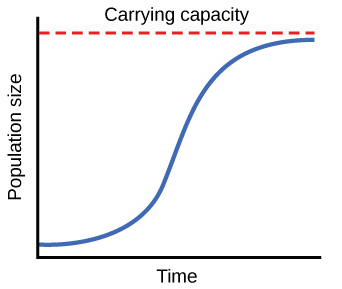
\includegraphics[width = \linewidth]{Logistic.jpg}
\caption{Logistic Curve}
\end{figure}

Here, $r$ is the Growth Rate and $k$ is the Carrying Capacity, or in other words, the max population that the existing resources can support.

\section{Experiment}

\subsection{Setup}

The experimental setup had {\em{Escherichia coli}} bacteria in different solutions in test-tubes.

The test-tubes had different pH values, as well as different nutrient concentrations.

So, we would be studying effect of carrying capacity and pH on growth of bacteria.

\subsection{Data Collection}

A Colorimeter was used to measure the ``absorption'' of the solutions for light of 540 nm wavelength.

Bacteria scatter light and do not allow light to reach the detector of the Colorimeter. So, if a solution has more bacteria, it is optically denser, scattering more light and hence giving a higher absorption reading.

This method allows us to very easily substitute Optical Density for actual population numbers. 


A limitation is that some amount of dead bacteria are also measured due to it. But, simplicity takes the priority here.


\section{Observation and Inference}

The graphs have been attached in a separate sheet. 

As far as the pH values go, it appears that neutral or slightly alkaline pH has a higher growth rate and higher carrying capacity. 

The graphs can be divided into three separate categories:

\begin{itemize}
    \item Original Nutrient Concentration, any pH
    \item 1:5 dilution, any pH
    \item 1:10 dilution, any pH
\end{itemize}

In each of the three categories, the growth rate and carrying capacities are nearly the same.

The carrying capacities being similar confirm to our model. Higher dilutions have lower carrying capacity as expected.


However, we would have expected all of them to show the same growth rate.

But, we see different values of $r$ for different nutrient dilutions. 

This shows a deviation from the Logistic Model. 

\textbf{A Possible Model}

$r$ may vary in a similar way as the Michelson Mentel Equation.

\[ 
    r = \frac{r_{max}[S]}{[S] + K_m}    
\]

where $[S]$ is the Nutrient Concetration, and $K_m$ is the Growth Rate at half the max value. 

So, we see that Growth of Bacteria can be modeled by various mathematical formulations. 

\end{document}